\documentclass[9pt, twoside, twocolumn]{extarticle}

%% Important... Define the proper path for font files!
\def\fontpath{../nature-font/}
\usepackage[lightmode]{../naturecustom}

% Please define \titletext, \abstracttext, \topic, \writtendate, \doctype, and \keywords
\newcommand{\titletext}{Topological Data Analysis: Merging Algebraic Topology with Machine Learning}
\newcommand{\abstracttext}{Topological Data Analysis (TDA) offers a novel framework for understanding the intrinsic geometric and topological structures within complex datasets. By leveraging concepts from algebraic topology, TDA provides tools such as persistent homology to capture multi-scale features that are often elusive to traditional statistical methods. This paper explores the integration of TDA into machine learning pipelines, highlighting how topological insights can enhance model robustness, interpretability, and performance, especially in high-dimensional and noisy data environments. We discuss foundational concepts, practical implementations, and potential applications, aiming to bridge the gap between abstract mathematical theory and practical machine learning solutions.}
\newcommand{\topic}{Computational Topology}
\newcommand{\writtendate}{\today}
\newcommand{\doctype}{Article}
\newcommand{\keywords}{Topological Data Analysis, Machine Learning, Algebraic Topology, Persistent Homology, Feature Extraction}

% --- Begin Document ---
\begin{document}
% --- Title and Author Info ---
\titleblock

%% START EDITING FROM HERE
    The exponential growth of data in various domains necessitates advanced analytical tools capable of uncovering hidden structures and patterns. Traditional machine learning techniques, while powerful, often struggle with high-dimensional, noisy, or incomplete data. Topological Data Analysis (TDA) emerges as a promising approach, utilizing principles from algebraic topology to study the "shape" of data. By focusing on the connectivity and continuity of data points, TDA provides a lens to capture global features that are invariant under continuous transformations, offering robustness against noise and perturbations. This paper delves into the synergy between TDA and machine learning, exploring how topological insights can be harnessed to improve data analysis and model performance

    \begin{figure}[htbp]
        \centering
        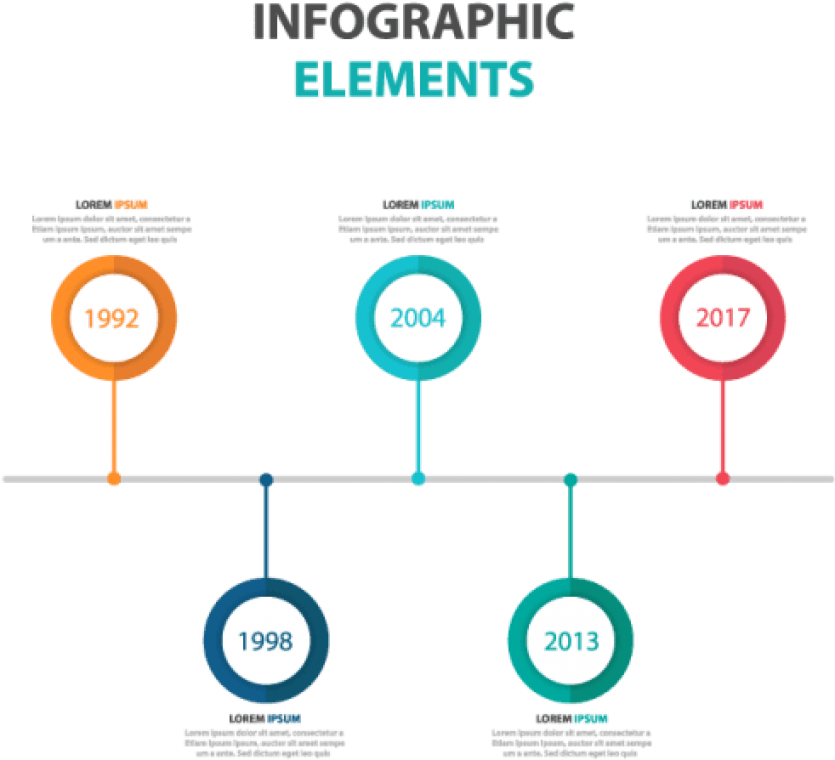
\includegraphics[width=0.8\linewidth]{diagram.png}
        \caption{Example figure caption.}
        \label{fig:example}
    \end{figure}


\section*{Foundations of Algebraic Topology in Data Analysis}

    \begin{table*}[t]
        \centering
        \begin{tabular}{|c|c|c|}
            \hline
            Dataset & Feature Representation & Topological Dimension \\
            \hline
            MNIST & Persistence Image & $\beta_1$ \\
            CIFAR-10 & Betti Curve & $\beta_0$, $\beta_1$ \\
            fMRI Brain Data & Persistence Diagram & $\beta_0$, $\beta_2$ \\
            Protein Graphs & Persistence Landscape & $\beta_1$ \\
            Synthetic Torus & Persistence Barcode & $\beta_1$, $\beta_2$ \\
            Financial Time Series & Betti Curve & $\beta_0$ \\
            Materials Microstructure & Persistence Image & $\beta_2$ \\
            Gene Expression & Persistence Diagram & $\beta_0$, $\beta_1$ \\
            \hline
        \end{tabular}
        \caption{Topological feature extraction methods applied across various datasets and their associated Betti dimensions.}
        \label{tab:tda_features}
    \end{table*}

    Topological Data Analysis (TDA) draws on core principles of algebraic topology to extract structural and shape-based features from data. This section outlines the mathematical foundations necessary for understanding how topology is applied to data, including the construction of simplicial complexes, the computation of homology, and the use of persistent homology for multi-scale analysis \cite{carlsson2009topology, hatcher2002algebraic, chazal2021introduction}.

    \subsection*{Simplicial Complexes and Filtrations}

        A \textbf{simplicial complex} is a combinatorial object that generalizes the notion of a graph to higher dimensions. Formally, a simplicial complex $K$ is a collection of finite sets closed under the subset operation: if $\sigma \in K$ and $\tau \subseteq \sigma$, then $\tau \in K$. Each $k$-dimensional simplex corresponds to a set of $k+1$ vertices:
        \[
        \sigma_k = [v_0, v_1, \dots, v_k], \quad \text{with } v_i \in V
        \]
        For data given as a point cloud $X = \{x_1, \dots, x_n\} \subset \mathbb{R}^d$, two common constructions are:

        \begin{itemize}
        \item \textbf{Vietoris-Rips Complex} $VR_\epsilon(X)$: includes a $k$-simplex for every set of $k+1$ points that are pairwise within distance $\epsilon$.
        \item \textbf{\v{C}ech Complex} $\check{C}_\epsilon(X)$: includes a $k$-simplex if the intersection of all balls of radius $\epsilon$ centered at the $k+1$ points is non-empty.
        \end{itemize}

        To analyze data at multiple scales, a filtration $\{K_\epsilon\}_{\epsilon \geq 0}$ is constructed:
        \[
        K_{\epsilon_0} \subseteq K_{\epsilon_1} \subseteq \cdots \subseteq K_{\epsilon_n}
        \]
        This filtration allows us to observe the birth and death of topological features as $\epsilon$ increases \cite{edelsbrunner2000topological}.

    \subsection*{Homology and Betti Numbers}

        Homology provides an algebraic summary of topological spaces by quantifying features such as connected components, loops, and voids. Given a simplicial complex $K$, we define:

        \begin{itemize}
            \item The $k$-th chain group $C_k(K; \mathbb{F})$ as the vector space over a field $\mathbb{F}$ spanned by the $k$-simplices of $K$.
            \item The boundary operator $\partial_k : C_k \to C_{k-1}$ satisfying $\partial_{k} \circ \partial_{k+1} = 0$.
        \end{itemize}

        The $k$-th homology group is then:
        \[
        H_k(K; \mathbb{F}) = \frac{\ker(\partial_k)}{\operatorname{im}(\partial_{k+1})}
        \]
        The dimension of $H_k$ is the $k$-th \textbf{Betti number} $\beta_k$, which intuitively counts:
        \begin{align*}
        \beta_0 &= \text{number of connected components} \\
        \beta_1 &= \text{number of independent loops} \\
        \beta_2 &= \text{number of voids or cavities}
        \end{align*}

        These numbers provide coarse yet powerful summaries of topological shape \cite{hatcher2002algebraic}.


    \subsection*{Persistent Homology}

        Persistent homology tracks the evolution of homology classes across a filtration. For each $k$-dimensional feature, we record its birth $\epsilon_b$ and death $\epsilon_d$ values:
        \[
        \text{Persistence Pair: } (\epsilon_b, \epsilon_d)
        \]

        These pairs are often visualized via:
        \begin{itemize}
            \item \textbf{Persistence Diagrams} $\mathcal{D}_k$: a multiset of points $(\epsilon_b, \epsilon_d) \in \mathbb{R}^2$ above the diagonal.
            \item \textbf{Barcodes}: horizontal lines spanning from $\epsilon_b$ to $\epsilon_d$ on a 1D axis.
        \end{itemize}

        The $p$-Wasserstein distance between two persistence diagrams $\mathcal{D}_1$ and $\mathcal{D}_2$ gives a notion of similarity between topological signatures:
        \[
        W_p(\mathcal{D}_1, \mathcal{D}_2) = \left( \inf_{\gamma: \mathcal{D}_1 \to \mathcal{D}_2} \sum_{x \in \mathcal{D}_1} \|x - \gamma(x)\|^p_\infty \right)^{1/p}
        \]
        where $\gamma$ is a bijection between diagrams (possibly allowing diagonal projections).

        Persistent homology distinguishes noise from signal by measuring the longevity of features: long intervals in barcodes often correspond to significant topological structure, while short ones indicate noise \cite{edelsbrunner2000topological, chazal2021introduction}.

        \begin{figure*}
            \centering
            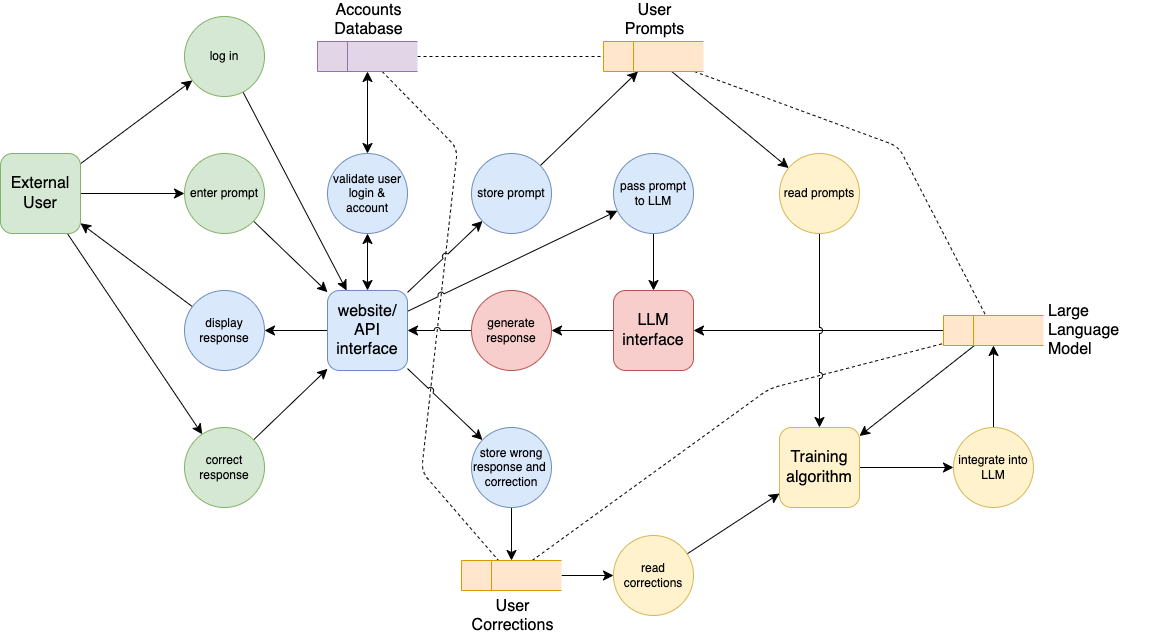
\includegraphics[width=\textwidth]{diagram-2.png}
            \caption{Example of a figure spanning two columns.}
            \label{fig:example-full}
        \end{figure*}

    \subsection*{Example: Circle and Torus}

        Consider data sampled from a noisy circle $S^1$. Its ideal homology is:
        \[
        \beta_0 = 1, \quad \beta_1 = 1, \quad \beta_k = 0 \text{ for } k > 1
        \]
        For a torus $T^2$, we expect:
        \[
        \beta_0 = 1, \quad \beta_1 = 2, \quad \beta_2 = 1
        \]
        TDA can recover these signatures even from scattered point clouds using persistent homology, providing strong evidence for underlying topological structure \cite{carlsson2009topology, rieck2020tda}.

\section*{Integrating TDA into Machine Learning}

    While persistent homology provides powerful topological summaries, its integration into machine learning workflows requires careful encoding, interpretation, and computational adaptation. This section outlines how topological features are translated into vectorized representations, used to improve model robustness, and applied across various domains \cite{hofer2017deep, rieck2020tda}.

    \subsection*{Feature Extraction and Representation}

        Persistence diagrams $\mathcal{D}_k$ are not naturally suited for direct consumption by standard machine learning algorithms due to their variable size and set-based nature. To bridge this gap, several techniques have been developed to convert diagrams into fixed-dimensional vector spaces:

        \begin{itemize}
            \item \textbf{Persistence Landscapes} \cite{bubenik2015statistical} represent $\mathcal{D}_k$ as a sequence of piecewise-linear functions:
            \[
            \lambda_k(t) = \sup_{(b,d) \in \mathcal{D}_k} \left[ \min\left( t - b, d - t \right)_+ \right]
            \]
            where $(\cdot)_+ = \max(\cdot, 0)$, giving a functional summary that supports statistical analysis in Banach spaces.

            \item \textbf{Persistence Images} \cite{adams2017persistence} map each diagram to a fixed-size grid with Gaussian kernels centered at each point $(b,d)$:
            \[
            \rho(x, y) = \sum_{(b,d) \in \mathcal{D}_k} \exp\left(-\frac{(x - b)^2 + (y - d)^2}{2\sigma^2}\right)
            \]
            This transforms topological features into image-like tensors that can be fed directly into neural networks or classifiers.

            \item \textbf{Betti Curves} plot Betti numbers over the filtration parameter $\epsilon$:
            \[
            \beta_k(\epsilon) = \text{rank}(H_k(K_\epsilon))
            \]
            giving a coarse yet intuitive descriptor for the evolution of topological complexity across scales.
        \end{itemize}

        These representations retain essential topological structure while conforming to the expectations of downstream models.

    \subsection*{Enhancing Model Robustness and Interpretability}

        Topological features provide complementary information to geometric and statistical features. In particular:

        \begin{itemize}
            \item \textbf{Robustness}: Persistent homology is stable under perturbations of the data \cite{chazal2021introduction}, meaning features with long lifespans persist even under noise. This makes topological descriptors ideal for noisy or incomplete datasets.
            \item \textbf{Global Structure Awareness}: Unlike local features (e.g., gradients or kernels), topological features capture global connectivity, loops, and voids—critical for problems where such structure encodes meaning, such as protein folding or brain connectivity.
            \item \textbf{Interpretability}: Betti numbers and persistence diagrams are human-interpretable. For instance, a significant $\beta_1$ feature may correspond to a loop in the data manifold—something that geometric embeddings like PCA would fail to express.
        \end{itemize}

        Recent work has shown that neural networks augmented with topological features, or trained using topologically-informed regularizers, exhibit improved generalization and adversarial resilience \cite{hofer2017deep, rieck2020tda}.

        \subsection*{Applications Across Domains}

        Topological data analysis has found practical utility in a wide range of scientific and industrial applications:

        \begin{itemize}
            \item \textbf{Biology}: In gene expression analysis, TDA captures clustering structures and loops in expression profiles that may correspond to cyclic biological processes or subpopulations \cite{carlsson2009topology}.
            \item \textbf{Neuroscience}: Persistent homology has been applied to functional MRI data to identify topological patterns in brain activity, such as connectedness and modularity of neural networks \cite{chazal2021introduction}.
            \item \textbf{Materials Science}: Topological fingerprints of porous structures in materials help in quantifying permeability and mechanical properties.
            \item \textbf{Finance}: TDA can detect regime changes and anomalous market behavior by capturing shape-based anomalies in high-dimensional stock trajectories \cite{rieck2020tda}.
        \end{itemize}

        These examples showcase TDA's versatility as a domain-agnostic tool for extracting meaningful structure in complex datasets.

\section*{Conclusion}

    Topological Data Analysis offers a powerful and mathematically principled approach to understanding the shape and structure of complex datasets. By leveraging concepts from algebraic topology—such as simplicial complexes, homology groups, and persistent homology—TDA provides a robust, noise-tolerant framework for uncovering multiscale geometric features that are often invisible to conventional statistical techniques \cite{carlsson2009topology, chazal2021introduction}.

    The integration of TDA into machine learning pipelines has opened new avenues for both theoretical exploration and practical application. Through persistence-based feature extraction methods like persistence landscapes, images, and Betti curves, topological summaries can be transformed into vectorized representations suitable for modern learning algorithms \cite{bubenik2015statistical, adams2017persistence}. These features enhance interpretability, improve robustness to noise and adversarial attacks, and often yield performance gains in settings where data is high-dimensional, sparse, or structured in nontrivial ways.

    Despite its potential, TDA faces several challenges that must be addressed for widespread adoption. Computational complexity, particularly in high dimensions, remains a bottleneck. Additionally, the interpretability of topological features across domains, as well as their seamless integration with deep learning architectures, are areas of active research \cite{hofer2017deep, rieck2020tda}.

    Nonetheless, as the field matures and software tools continue to evolve, the application of topological methods in machine learning is expected to grow significantly. The synergy between rigorous mathematical abstraction and practical data analysis embodied by TDA is emblematic of a broader trend—where geometry, topology, and learning theory converge to create next-generation analytical tools.


% --- Mandatory Acknowledgements for Font---
\fontacknowledgment
% --- References (Example) ---
\bibliographystyle{abbrv}
\bibliography{references}

\end{document}
